\subsection{Analysis}
\label{sec:analysis}
\begin{figure*}[h]
\centering
\begin{minipage}[t]{0.40\textwidth}
\centering
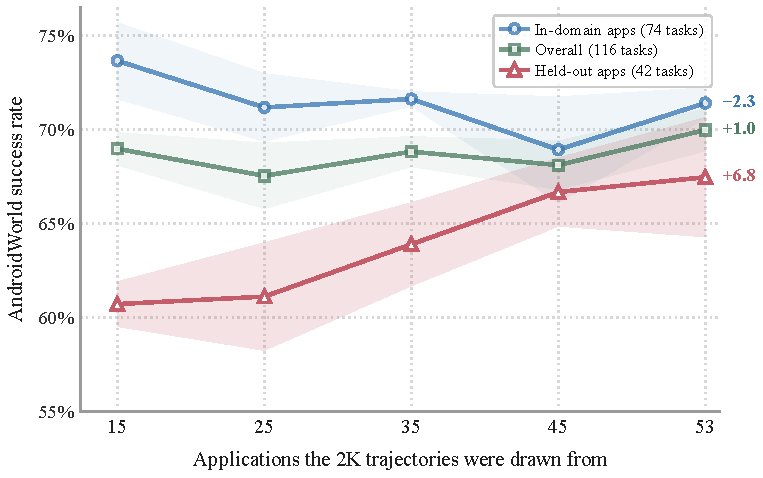
\includegraphics[
    width=\linewidth,
    keepaspectratio
]{figures/exp-env-scaling.pdf}\\[-0.2em]
{\small (a) Environment coverage}
\end{minipage}
\hfill
\begin{minipage}[t]{0.56\textwidth}
\centering
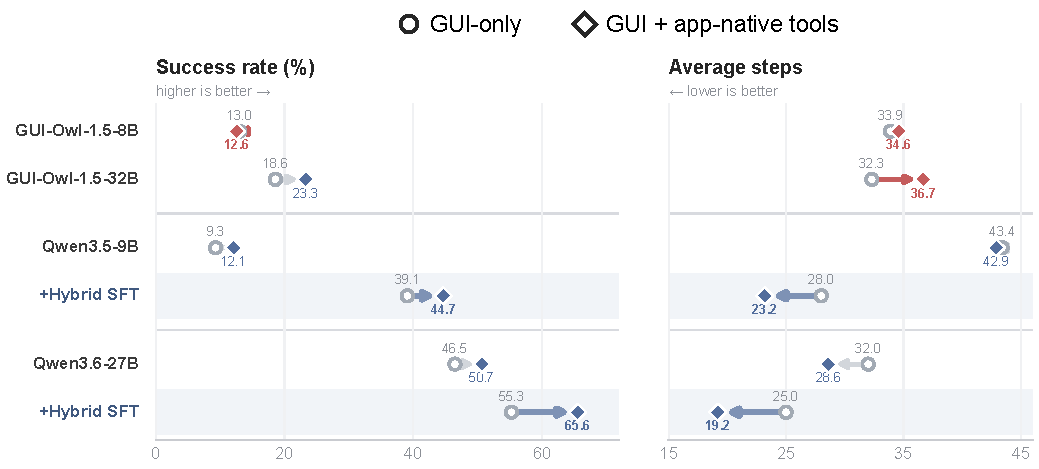
\includegraphics[
    width=\linewidth,
    keepaspectratio
]{figures/exp_tool_analysis_old.pdf}\\[-0.2em]
{\small (b) App-native tool use}
\end{minipage}
\caption{
\textbf{Environment coverage and app-native tool use.}
(a)~Broader coverage improves held-out AndroidWorld performance at a fixed 2K-trajectory budget.
(b)~App-native tools improve success and efficiency, with larger gains after Hybrid SFT.
}
\label{fig:analysis-results}
\end{figure*}

We focus our analysis on two aspects of mobile agent interaction: how environment coverage relates to generalization, and how app-native tools complement GUI interaction.






\paragraph{Broader environment coverage improves transfer under a fixed data budget.}
With the backbone, optimizer, and total training data fixed at 2K emulator
trajectories, we vary application coverage from 15 to 53 while keeping the
same 15 InD applications. Broader coverage improves transfer to unseen
applications, with Pass@1 increasing from 60.7 to 67.5 (Figure~\ref{fig:analysis-results}a).
Meanwhile, the InD data share drops from 100\% to 39.1\%, but InD Pass@1
remains largely stable (73.7$\rightarrow$71.4; Table~\ref{tab:env-split}).
These results show that broader application coverage improves generalization
without significantly compromising performance on familiar applications.

\begin{table}[h]
\centering
\small
\begin{minipage}[t]{0.33\linewidth}
\centering
\caption{
Environment-coverage settings under a fixed budget of 2K trajectories. InD share denotes the fraction of training trajectories from the 15 in-distribution applications.
}
\label{tab:env-split}
\setlength{\tabcolsep}{3pt}
\begin{tabular}{cc}
\toprule
\# Train apps & InD data share \\
\midrule
15 & 100\% \\
25 & 64.0\% \\
35 & 48.9\% \\
45 & 41.1\% \\
53 & 39.1\% \\
\bottomrule
\end{tabular}
\end{minipage}
\hfill
\begin{minipage}[t]{0.63\linewidth}
\centering
\caption{App-native tool use on MobileGym++.
TR (tool-call rate) is the average number of app-native tool calls per task. \#Tools is the number of distinct tools invoked across the benchmark, and \#Tasks is the number of tasks (out of 215) in which at least one app-native tool is called.}


\label{tab:tool_use}
\setlength{\tabcolsep}{3pt}
\resizebox{0.76\linewidth}{!}{%
\begin{tabular}{llccc}
\toprule
Model & Stage & TR & \#Tools & \#Tasks \\
\midrule
GUI-Owl-1.5-8B &- &0.58&15&20\\
GUI-Owl-1.5-32B &- &0.51&51&45\\
\midrule
\multirow{2}{*}{Qwen3.5-9B} & Base & 0.64 & 28 & 21 \\
 & + Hybrid SFT & 1.41 & 110 & 113 \\
\midrule
\multirow{2}{*}{Qwen3.6-27B} & Base & 1.64 & 97 & 102 \\
 & + Hybrid SFT & 2.23 & 115 & 128 \\
\bottomrule
\end{tabular}%
}
\end{minipage}
\end{table}


\paragraph{Hybrid training unlocks the benefits of app-native tools.}
Providing app-native tools alone does not guarantee effective tool use: without hybrid training, models rarely learn when to invoke them.
Before hybrid SFT, tool calls appear in only 20--102 of 215 tasks (Table~\ref{tab:tool_use}), bringing limited gains: Qwen models improve by only 2.8--4.2 points, while GUI-Owl-1.5 shows inconsistent results and can even degrade (Figure~\ref{fig:analysis-results}b).
After hybrid SFT, tool usage becomes substantially more effective: tool calls appear in 113 and 128 tasks, covering 110 and 115 distinct tools for the 9B and 27B models, respectively. More importantly, tool-enabled gains increase to 5.6 and 10.3 points, while trajectories become 4.8 and 5.8 steps shorter. These results show that hybrid training teaches models to effectively leverage app-native tools, improving both task success and interaction efficiency.
